\documentclass[12pt]{article}
\usepackage{amsmath,amssymb,amsthm}
\usepackage{graphicx}
\usepackage{float}
\usepackage{geometry}
\geometry{top=1in, bottom=1.25in, left=1in, right=1in}
\usepackage{caption}
\usepackage{subcaption}
\usepackage{pdfpages}
\usepackage{hyperref}
\usepackage{gensymb}
\hypersetup{
    colorlinks=true, 
    linkcolor=black, 
    urlcolor=blue,
    pdftitle={Project 1: Heating and Cooling of Buildings},
    pdfauthor={William Roberts, Ryan Jenkins, Evan Miller}
}
\usepackage{booktabs}
\usepackage{array}
\usepackage{mathtools}
\usepackage{bm}
\usepackage{siunitx}
\usepackage{enumitem}
\usepackage{listings}
\usepackage{xcolor}

\lstset{
  language=Matlab,
  basicstyle=\ttfamily\small,
  keywordstyle=\color{blue},
  commentstyle=\color{green!50!black},
  stringstyle=\color{orange},
  breaklines=true,
  breakatwhitespace=true,
  showstringspaces=false,
  frame=single,
  captionpos=b,
  numbers=left,           
  numberstyle=\small\color{black},  
  stepnumber=1,        
  numbersep=10pt 
}


\setlist{nosep}

\title{Project 1: Heating and Cooling of Buildings}
\author{William Roberts \and Ryan Jenkins \and Evan Miller}
\date{\today}

\begin{document}
\maketitle

\tableofcontents
\clearpage

\section{Introduction}
Billy Bob works in a specialized laboratory dedicated to studying microbial cells, where maintaining precise temperature conditions is crucial. Each day, he monitors the building’s heating and cooling systems to ensure that the microbes are kept within safe temperature ranges. Even small fluctuations in temperature could compromise experiments or damage sensitive equipment. To better understand how the indoor environment responds to various influences, Billy Bob decides to investigate the factors that control the lab's temperature. He considers the impact of the outside weather, the heat generated by internal sources, and the role of the thermostat in maintaining a stable environment for the laboratory. By combining analytical modeling with numerical simulations, he aims to predict temperature changes, identify potential risks, and develop strategies to keep the lab conditions safe and consistent.

\section{Background}
For the purposes of modeling the temperature of the building, $T$, at time $t$. The three elements Billy Bob is looking at are: the effect of the ambient outside temperature, $A(t)$, the heat produced by machinery, lights, and people, $H(t)$, and artificial heating and cooling, $Q(t)$, yielding the differential equation $ \frac{dT}{dt} = A(t) + H(t) + Q(t)$ (1).

\section{Analytical investigation (Task Set A)}
We begin with the general model
\begin{equation}
\frac{dT}{dt} = \kappa \big(M(t) - T(t)\big) + H(t) + Q(t).
\label{eq:general}
\end{equation}
This is a first–order, linear, non–homogeneous ODE. Since $M(t)$, $H(t)$, and $Q(t)$ may depend on time, the equation can have variable coefficients. If $Q(t)=tT$, then the equation would no longer be linear due to the product $tT$. By Picard’s Theorem, existence and uniqueness of solutions are guaranteed if the right–hand side of the ODE is continuous in $t$ and Lipschitz continuous in $T$. These conditions are satisfied if $M(t)$, $H(t)$, and $Q(t)$ are continuous, so the model has a unique solution for any given initial condition. Physically, this means the building’s indoor temperature trajectory is completely determined once $T(0)$ is specified. To solve analytically, we rewrite the ODE in standard form,
\begin{equation}
\frac{dT}{dt} + \kappa T = \kappa M(t) + H(t) + Q(t).
\label{eq:standard}
\end{equation}
Using the integrating factor $\mu(t) = e^{\kappa t}$, we obtain
\begin{equation}
\frac{d}{dt}\big(e^{\kappa t}T(t)\big) = e^{\kappa t}\big(\kappa M(t) + H(t) + Q(t)\big),
\label{eq:IFderiv}
\end{equation}
and integrating gives
\begin{equation}
T(t) = e^{-\kappa t}\left(\int e^{\kappa t}(\kappa M(t) + H(t) + Q(t))\,dt + C\right),
\label{eq:integralsol}
\end{equation}
where $C$ is determined by the initial condition. In the special case where $H(t)=0$ and $Q(t)=0$ with constant exterior temperature $M(t)=M_0$, the model reduces to
\begin{equation}
\frac{dT}{dt} = \kappa(M_0 - T).
\label{eq:constantM}
\end{equation}
The equilibrium solution is $T=M_0$. This equilibrium is stable, since the temperature moves toward $M_0$ whether it starts above or below. Solving the IVP with $T(0)=T_0$ yields
\begin{equation}
T(t) = M_0 + (T_0 - M_0)e^{-\kappa t}.
\label{eq:closed}
\end{equation}

We first set $\kappa=0.25$ and $M_0=75$, and compare solutions with initial conditions $T(0)=0$, $50$, and $80$. As shown in Figure~\ref{fig:TaskA1}, all solutions converge to the equilibrium $T=75^\circ$. 

\begin{figure}[H]
    \centering
    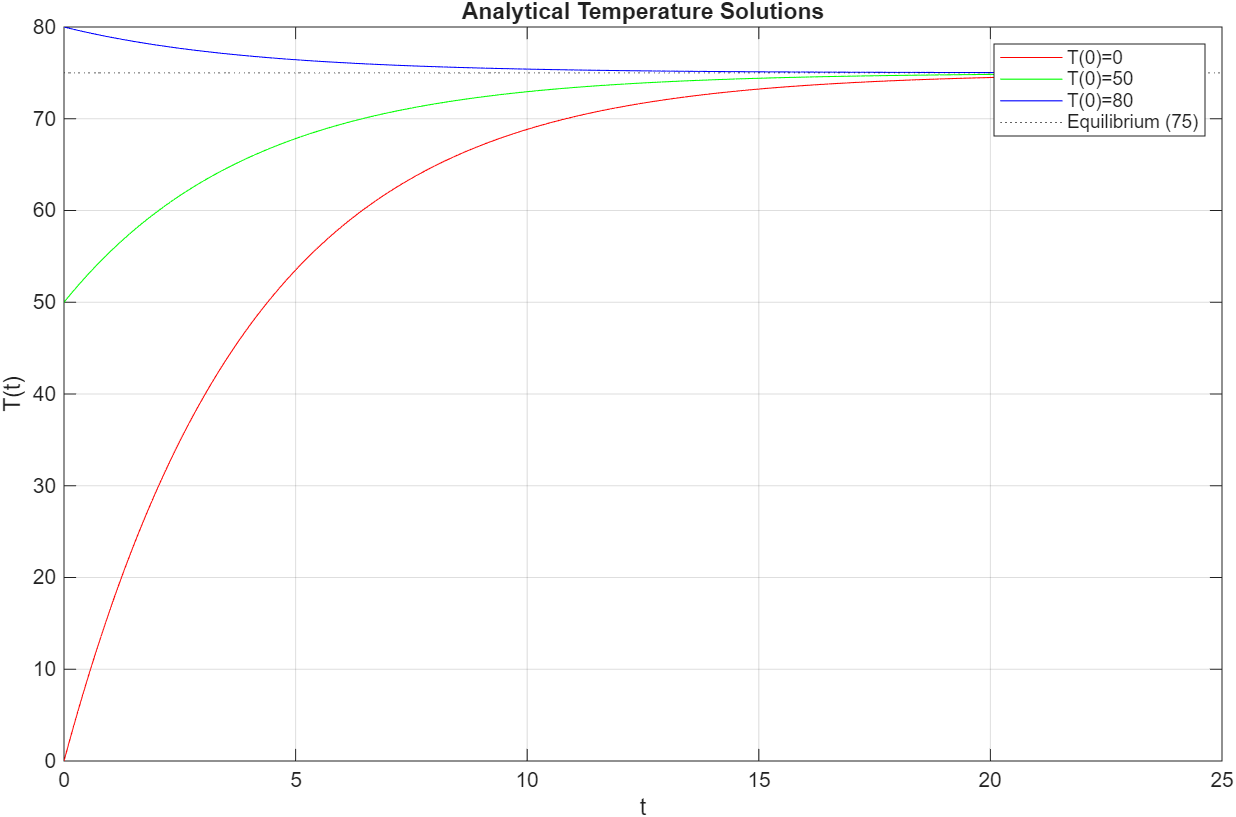
\includegraphics[width=0.75\linewidth]{images/Task_A1.png}
    \caption{Analytical solutions with $\kappa=0.25$, $M_0=75$, and varying initial conditions.}
    \label{fig:TaskA1}
\end{figure}

Next, we fix $M_0=75$ and $T(0)=50$ while varying $\kappa=1.0,\,0.5,\,0.25$. Figure~\ref{fig:TaskA2} shows that larger $\kappa$ values result in faster convergence to equilibrium. Physically, $\kappa$ controls how quickly the building’s interior temperature responds to the outdoor temperature.

\begin{figure}[H]
    \centering
    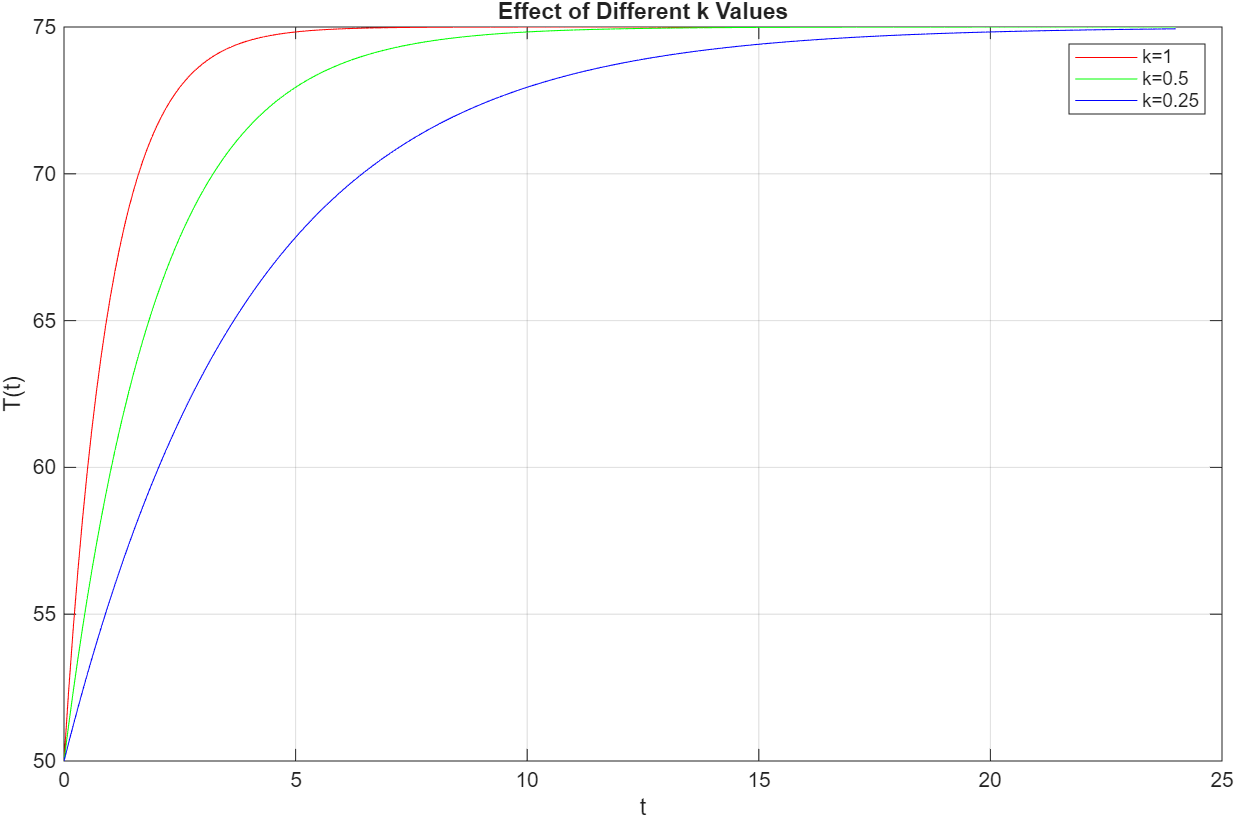
\includegraphics[width=0.75\linewidth]{images/Task_A2.png}
    \caption{Effect of different $\kappa$ values on convergence rate to equilibrium.}
    \label{fig:TaskA2}
\end{figure}
We can also determine the time required for the difference between the inside and outside temperatures to decay to $e^{-1}$ of its initial value. From the solution,
\begin{equation}
T(t) = M_0 + (T_0 - M_0)e^{-\kappa t},
\label{eq:closed_repeat}
\end{equation}
the distance from equilibrium is given by $|T(t)-M_0| = |T_0 - M_0|e^{-\kappa t}$. Requiring this to equal $|T_0 - M_0|e^{-1}$ yields
\begin{equation}
e^{-\kappa \Delta t} = e^{-1},
\end{equation}
so $\kappa \Delta t = 1$ and hence
\begin{equation}
\Delta t = \frac{1}{\kappa}.
\label{eq:timeconst}
\end{equation}

This quantity is called the time constant, with units of hours. For the values of $\kappa$ considered previously, the time constants are $1$, $2$, and $4$ hours when $\kappa = 1,\,0.5,\,0.25$, respectively. A larger time constant corresponds to a slower response of the building’s temperature to outside fluctuations, reflecting greater thermal stability, while a smaller time constant indicates quicker adjustment.


\section{Numerical methods and verification (Task Set B)}

When using simplified versions of the temperature model, as was the case in the previous section, where $H(t)$ and $A(t)$ are assumed to be zero and $M(t)$ is assumed constant, the differential equation modeling the internal building temperature can be solved by hand. However, as the model improves, considering the effects of more of these variances, it will become impractical to perform these calculations manually. As such, it is pertinent to develop and verify a program to numerically approximate solutions to these models, in this case, the fourth-order Runge-Kutta program featured in Appendix A.

In order to test our program and verify its accuracy, we can plug in equation (?) and compare the results to the exact solution obtained in the previous section. Plotting the solutions against each other in Figure 3, we can compare the two solutions.

\begin{figure}[H]
     \centering
    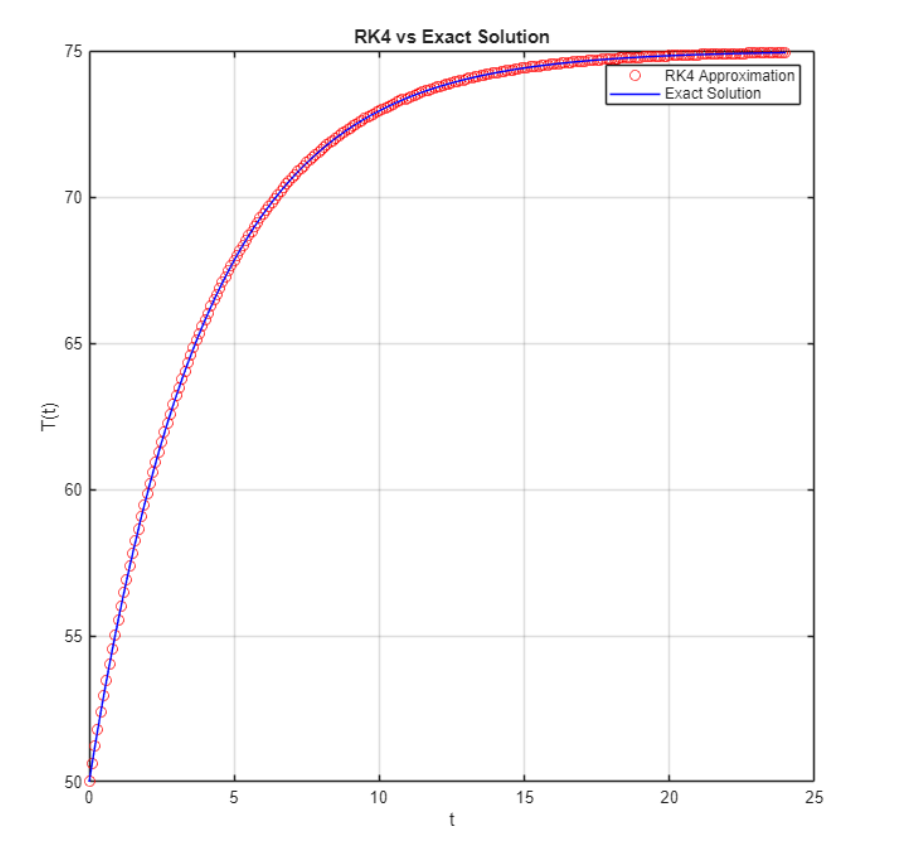
\includegraphics[width=0.75\linewidth]{images/Task_B1.png}
    \caption{Runge-Kutta fourth-order approximation vs exact solution}
    \label{fig:placeholder}
\end{figure}
   

To quantify this comparison, refer to Figure 4, plotting the error in our approximation. 

\begin{figure}[H]
    \centering
    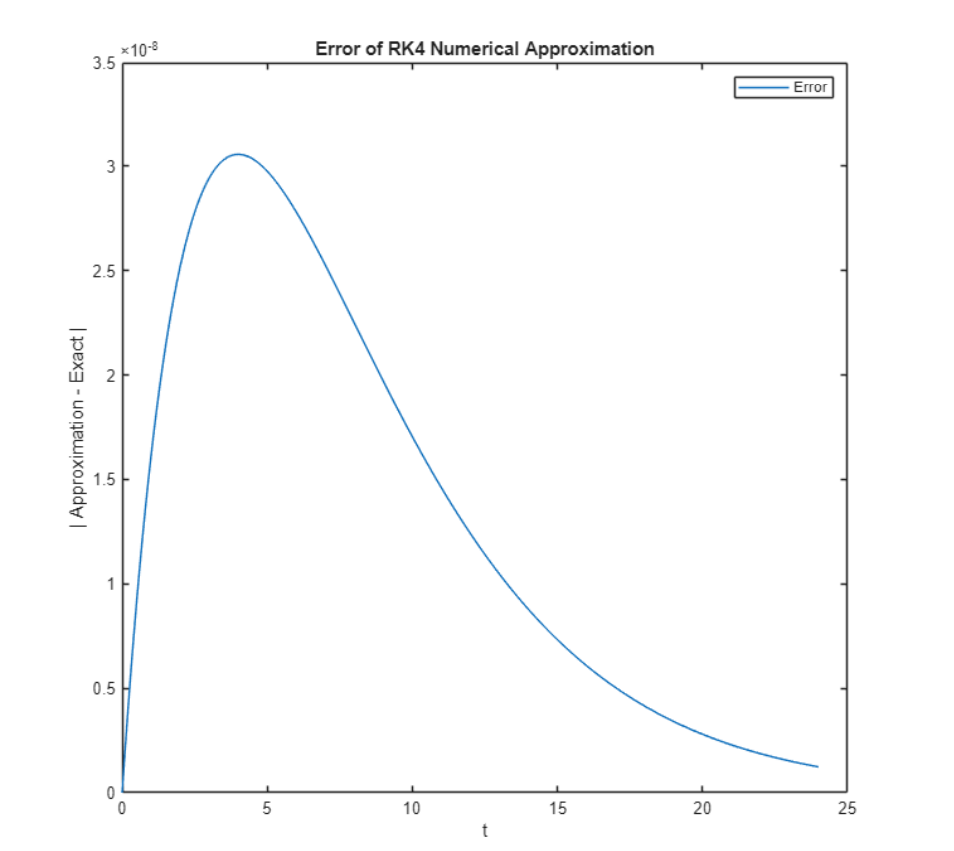
\includegraphics[width=0.75\linewidth]{images/Task_B2.png}
    \caption{Runge-Kutta Error}
    \label{fig:placeholder}
\end{figure}

Because the error displayed here peaks at about $(3.06\times10^-8)\degree$, we will consider our numerical solution a very good approximation of the actual solution, and use it for calculations going forward. 


\section{Refined models and simulations}
Now that we have a proven method for numerically solving the ODEs facing us, it is time to begin developing and refining our model into an accurate and useful tool for Billy's lab.
\subsection{Varying outside temperature (Task Set C)}
 To start with, we can replace the constant exterior temperature with the varying model, $M(t) = M_0 - 12cos(\frac{\pi(t-5)}{12})$ (5). Plugging M(t) into Equation 3 with initial conditions $M_0 = 75$ and $T(0)=65$, and numerically solving for $T(t)$ models the temperature inside the laboratory based on a varying outside temperature starting at $75\degree$ when the interior temperature starts at $65\degree$. The plot of the solution $T(t)$ alongside $M(t)$ yields Figure 5, showing the relationship between the external temperature and the internal temperature. 
\begin{figure}[H]
    \centering
    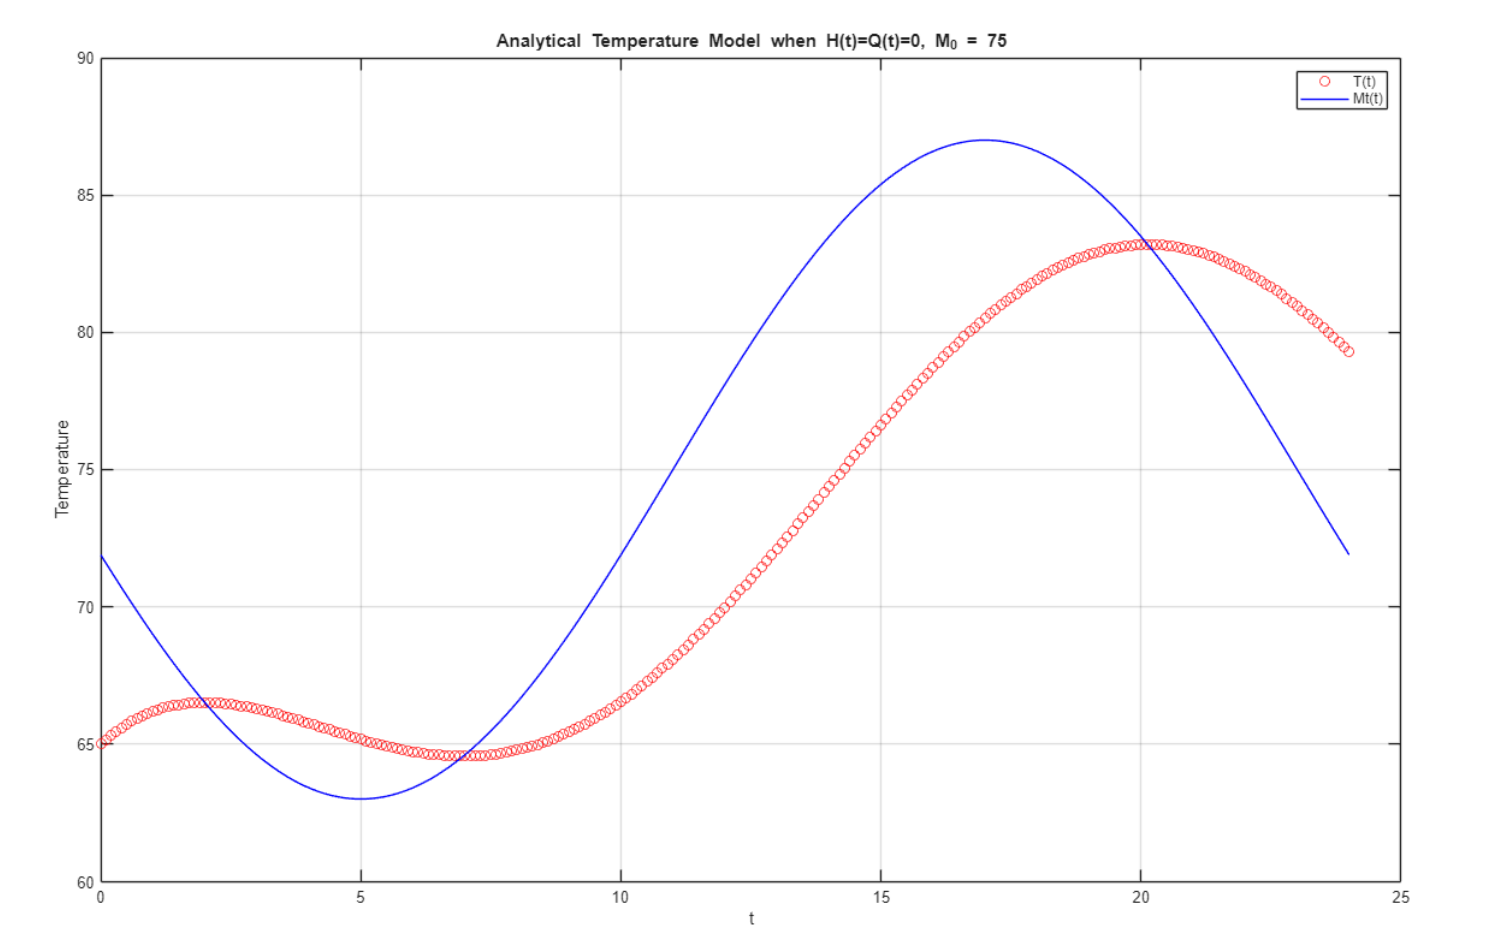
\includegraphics[width=0.75\linewidth]{images/Task_C1.png}
    \caption{Interior temperature vs exterior temperature when $M_0=75$}
    \label{fig:placeholder}
\end{figure}
When $M_0 = 75$, the temperature outside the lab will reach its peak of $87\degree$ at 17:00 and its minimum of $63\degree$ at 5:00, while the temperature inside the lab peaks to $83.19\degree$ at 20:06 and reaches a minimum of $64.56\degree$ at 7:00.

Repeating this process when the starting outside temperature, $M_0$, is instead $35\degree$, produces Figure 6 that compares the interior temperature and the outside temperature in this new condition. 
\begin{figure}[H]
    \centering
    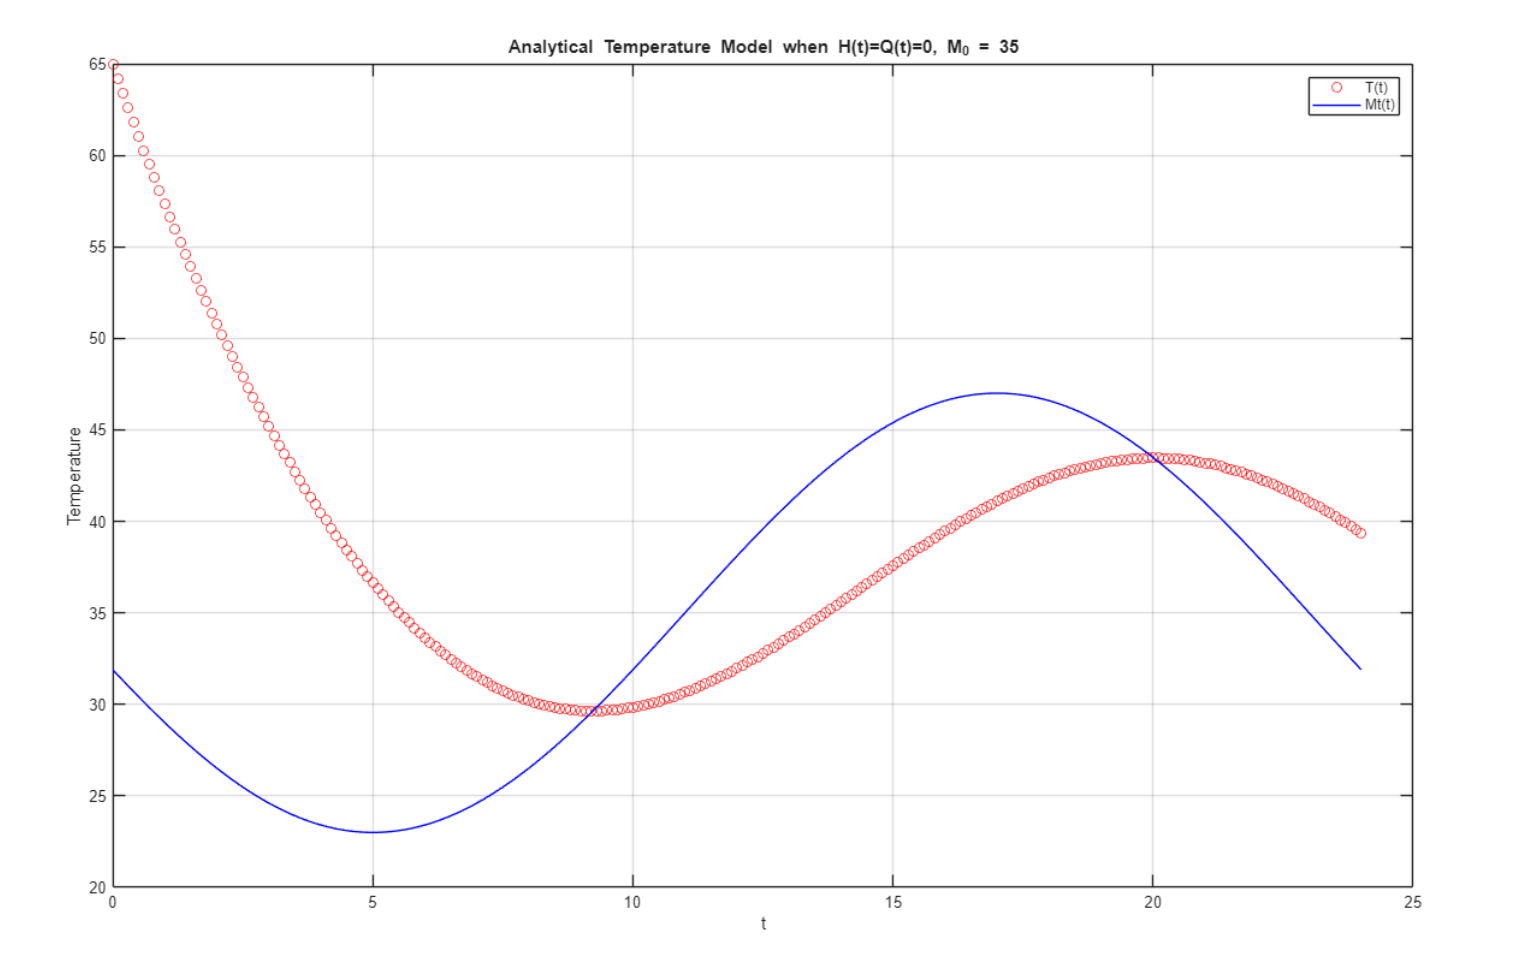
\includegraphics[width=0.75\linewidth]{images/Task_C2.png}
    \caption{Interior temperature vs exterior temperature when $M_0=35$}
    \label{fig:placeholder}
\end{figure}
Now, the temperature outside the lab will peak at $47\degree$ at 17:00 and reach a minimum of $23\degree$ at 5:00, while the highest temperature inside the lab is $65\degree$ right when the model starts at 0:00 and drops to a minimum of $29\degree$ at 9:12.

Figure 5 and Figure 6 show that the interior temperature reacts to the exterior temperature, continuously approaching it with a rate of change proportional to the difference between the two temperatures. In this manner, the inside temperature is always moving towards system equilibrium, where the outside and inside temperatures are equal. 

\subsection{Internal heat sources (Task Set D)}
Next, we can again modify Equation (3) to model the effect of heat produced by people, lights, and machinery within the lab on the inside temperature. For now, we will ignore the outdoor temperature and artificial heating and cooling influences to focus solely on the H(t) component of Equation (1). We can use the equation $H(t)=7sech[\frac{3}{4}(t-10)]$ (6) to model the heat produced by these factors, and plug this formula into Equation (3). From here, we can numerically solve and plot $T(t)$ based on $H(t)$, producing Figure 7.
\begin{figure}[H]
    \centering
    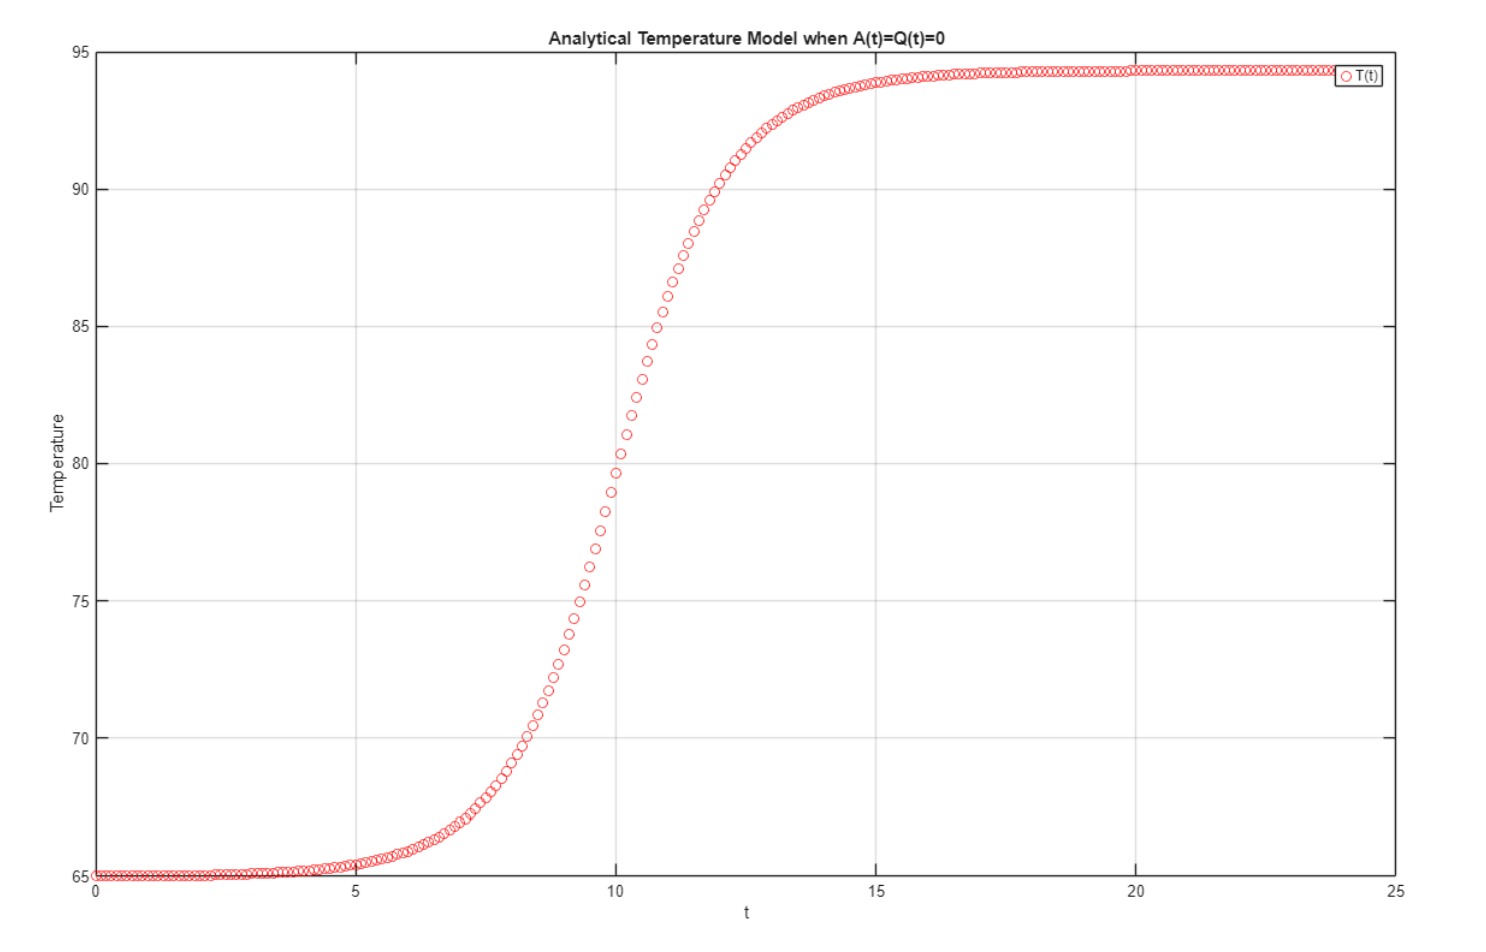
\includegraphics[width=0.75\linewidth]{images/Task_D1.png}
    \caption{Inside Lab Temperature from Lights, People, and Machinery}
    \label{fig:placeholder}
\end{figure}

We can also plot $H(t)$ itself, the heat being produced by people, lights, and machinery at time, $t$, shown here in Figure 8.
\begin{figure}[H]
    \centering
    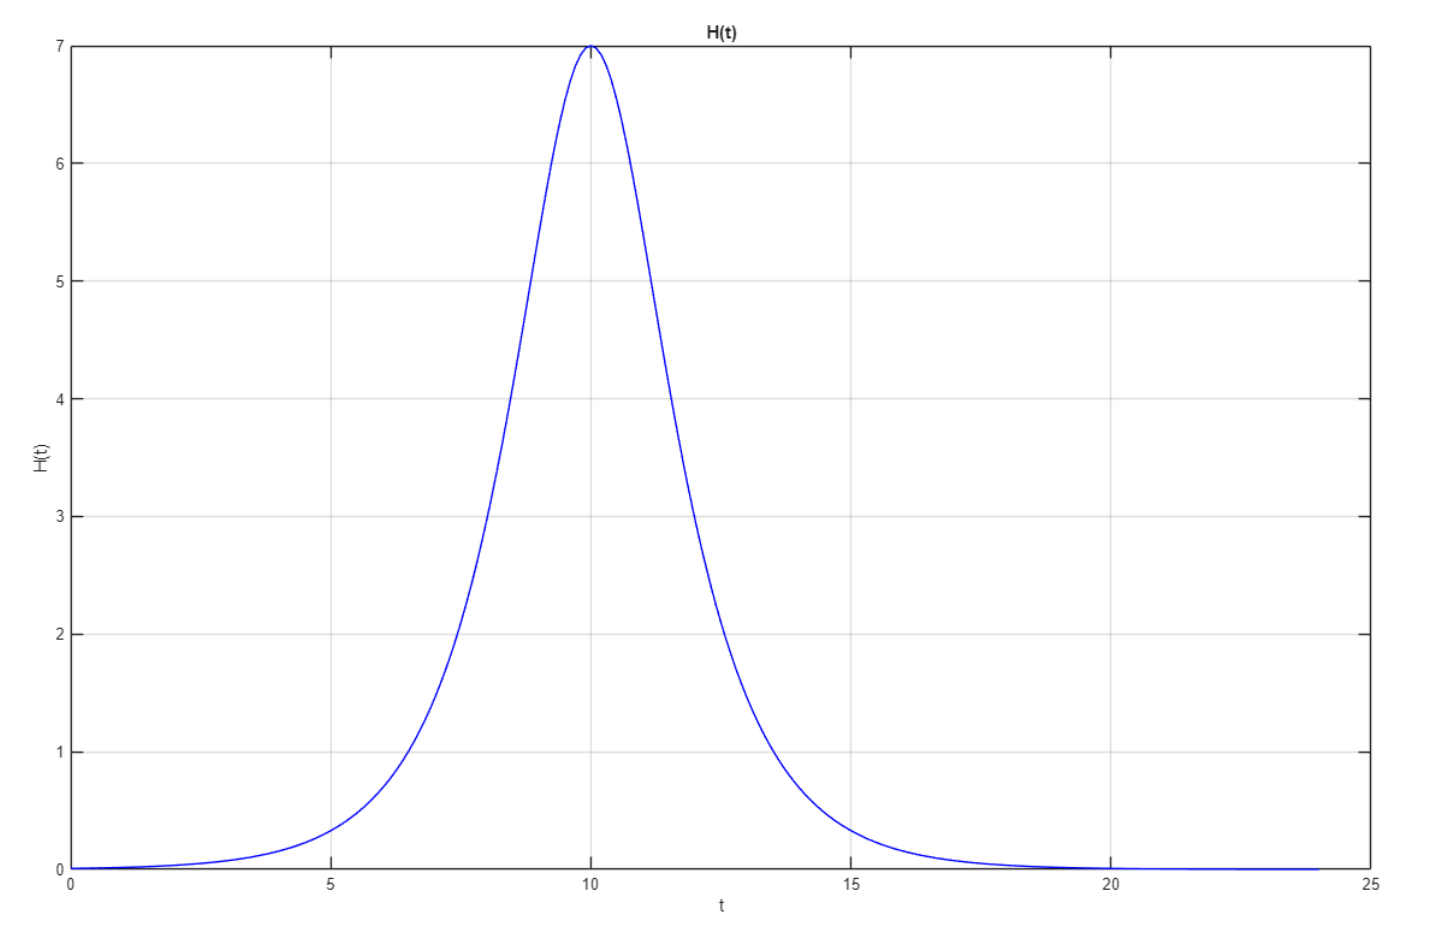
\includegraphics[width=0.75\linewidth]{images/Task_D2.png}
    \caption{H(t)}
    \label{fig:placeholder}
\end{figure}

From Figure 7, we can see that the temperature inside the lab reaches its peak of $94.31\degree$ at 24:00, the very end of the modeling period. Since $H(t)$ here represents the amount of heat being produced by machinery, lights, and people, at time, $t$, Figure 8 shows that Billy's lab is active primarily between the hours of 5:00 and 15:00, reaching peak activity at 10:00. This plot of $H(t)$ therefore explains the nature of $T(t)$, the solution of the differential equation. $H(t)$ is always positive and approaches zero at the start and end of each day, peaking the middle at 10:00. $H(t)$ corresponds to the rate of change, or slope, of $T(t)$, so the graph of $T(t)$ should be continuously increasing, with a flat slope at the start and end of the day, and steepest slope at 10:00. This corresponds perfectly with the plot of $T(t)$ in Figure 7.

\subsection{Thermostat control (Task Set E)}
To model the effect of furnaces and air conditioners we assume the thermostat provides heating or cooling proportional to the error between the desired temperature and the current temperature. We write
\begin{equation}
Q(t)=\kappa_d(T_d-T)
\label{Qthermostat}
\end{equation}
and, taking $A(t)=H(t)=0$ in the general model \eqref{eq:general}, the governing initial value problem becomes,
\begin{equation}
\frac{dT}{dt} = \kappa_d(T_d - T), \qquad T(0)=T_0
\label{eq:thermostat_ode}
\end{equation}
This has the explicit solution
\begin{equation}
T(t)=T_d+(T_0-T_d)e^{-\kappa_dt}
\label{eq:thermostat_solution}
\end{equation}
so the controlled dynamics are exponential with time constant $1/\kappa_d$.

\section{Combined scenarios and safety analysis (Task Set F)}
In some of the previously modeled scenarios, particularly the model of $T(t$
\clearpage
\section{Results}

\section{Conclusion}

\clearpage
\appendix
\section{Appendix A: Code}
\lstinputlisting{code/tasks.m}


\section{Appendix B: Lengthy Calculations}


\end{document}




